\section{Performance Introspection}\label{sec:framwework}

\begin{figure}
    \centering
    \setlength{\belowcaptionskip}{-10pt}
    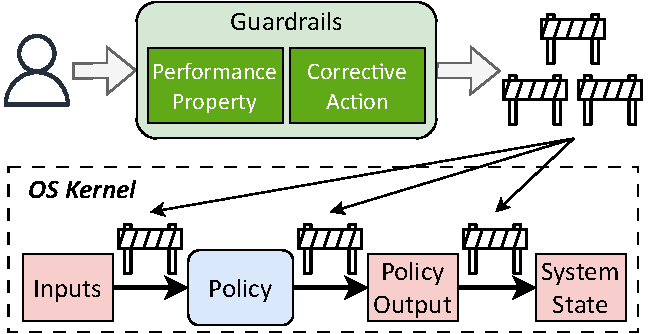
\includegraphics[width=0.8\columnwidth]{figures/Overview/overview.pdf}
    \caption{Overview of Guardrails}
    \label{fig:framework-overview}
\end{figure}

%Today, the general approach operators use to detect performance degradations like the ones shown in Section~\ref{sec:motivating} \aditya{what is this referring to} is via extensive offline evaluation across a wide range of workloads, followed by manual inspection of end-to-end performance metrics. This process is tedious, incomplete, and ultimately unsatisfactory: no finite offline evaluation can anticipate the diversity of executions encountered in deployment.

% The examples in Section~2 highlight a recurring gap in current OS policy design. Even when a policy depends on quantities whose usefulness can drift at deployment time, the system typically lacks a built-in mechanism to monitor the relevant run-time evidence and react when that evidence suggests the policy is no longer operating in its intended regime. 
We argue for a new system capability, \emph{performance introspection}: the ability to specify run-time checks over policy-relevant observations, associate those checks with corrective actions, and relate such local mechanisms to broader performance goals.
We present a framework for run-time performance introspection in the OS, built around \emph{OS guardrails}. We summarize the framework here and develop the  abstractions in \Cref{sec:guardrails}. It has three components (Figure~\ref{fig:framework-overview}): a specification interface for expressing guardrails, a verification interface for relating them to high-level objectives, and system support for run-time monitoring and enforcement. % them at run time.

%In this paper, we propose a framework that brings such run-time performance introspection capabilities to the OS. The key building blocks enabling this framework are {\it \textbf{OS Guardrails}}.
%\eric{I don't like this sentence--Isn't the framework guardrails?}
%We provide an overview of our framework here, and discuss the core abstraction in \Cref{sec:guardrails}.
%As shown in Figure~\ref{fig:framework-overview}, the framework comprises three components: a specification interface for expressing guardrails, a verification interface for relating guardrails to high-level performance objectives, and system support for monitoring and enforcing guardrails at run time.
% In this section, we present our \emph{performance introspection} framework, which addresses the common need illustrated by the motivating:

\paragraph{Specification.}
For each policy or subsystem of interest, the framework allows a developer or operator to specify a \emph{guardrail}: a run-time condition that should hold during execution, together with a response to trigger when that condition is violated. Guardrails are written in the \emph{Guardrail Description Language (\lang)}, a domain-specific language for expressing checks and actions over kernel-visible signals. The purpose of \lang is to make guardrails both expressive enough to capture policy-specific behavior and structured enough to support efficient run-time monitoring.

\paragraph{Validation.}
Guardrails are inherently local: their conditions must be evaluated at run time and therefore can depend only on execution-time signals. In contrast, the OS policy designer often cares about a more global performance objective, such as avoiding regression relative to a default policy or preserving acceptable decision quality. To capture this distinction, the framework also allows the operator to specify a high-level performance objective, denoted \perfsafety in \Cref{fig:framework-overview}.
A verifier then checks, under a model of policy--system interaction ($M$ in \Cref{fig:framework-overview}), whether the guardrail condition and its prescribed response are sufficient to support the desired \perfsafety objective. This verification step is optional, but it provides a way to reason about whether a local guardrail serves the larger goal that motivated it.

\paragraph{Execution.}
At deployment time, the specified guardrails are compiled into \emph{Guardrail Monitors} that operate alongside the policy execution path. As the policy receives inputs, makes decisions, and updates system state, these monitors evaluate the corresponding run-time conditions over the resulting execution trace. We implement these monitors using \texttt{eBPF}, which enables low-overhead in-kernel execution and dynamic updates to the monitoring logic. When a guardrail condition fails, the monitor triggers the prescribed response. Depending on the guardrail, this response may update a parameter, switch to an alternative policy, fall back to a safer default, or simply record the violation for later diagnosis.


% \subsection{The OS Guardrail Abstraction}\label{subsec:guardrails-desc}




% \subsection{Running Examples}\label{subsec:guardrail-examples}

% We use two running examples to illustrate guardrails and the general performance introspection framework. 

% \paragraph{CBMM hugepage promotion.}
% Our first example is a hugepage-promotion policy based on CBMM~\cite{cbmm-atc22}. Hugepages can reduce TLB pressure and improve address-translation performance, but promoting them also incurs allocation and compaction costs. CBMM addresses this tradeoff by estimating, for each candidate promotion, whether the expected benefit of promotion exceeds its expected cost, and promoting a hugepage only when that inequality holds. This design creates a natural failure mode: the benefit estimates used by the policy may become inaccurate at deployment time as access patterns change. A guardrail for CBMM can therefore monitor whether the signals underlying these benefit estimates continue to track the observed behavior of promoted hugepages. If that condition fails, the corrective action may update the relevant benefit parameters using recently observed accesses. Under an appropriate system model, one can then ask whether such updates preserve a desired \perfsafety objective, such as avoiding regressions in promotion quality.

% \paragraph{Flow-size prediction for scheduling.}
% Our second example is the flow-size predictor shown in \Cref{fig:flux-example}. Here, a neural network predicts the size of each new flow, and the prediction is used for priority-based scheduling. A natural guardrail condition is that the predictor should only be used on inputs that are in-distribution with respect to its training data. When this condition fails, the corrective action may switch to another model or to a more conservative scheduling policy. As in the previous example, the verification interface can then be used to reason about whether this local repair is sufficient to preserve a higher-level objective, such as maintaining acceptable decision quality.
